\documentclass[]{article}
\usepackage{amsmath,amssymb}
\usepackage[letterpaper, margin=1in]{geometry}
\usepackage[final]{graphicx}
\usepackage{empheq}
\usepackage{tikz}
\usetikzlibrary{calc}


\pgfkeys{
  mygrid/.is family,
  mygrid,
  min x/.initial=-5,
  max x/.initial=5,
  min y/.initial=-5,
  max y/.initial=5,
  small step/.initial=.1,
  step/.initial=1,
  big step/.initial=5,
  color/.initial=red,
}
\newcommand\mygridset[1]{\pgfkeys{mygrid,#1}}
\newcommand\mygrid[1][]{
  \mygridset{#1,
    min x/.get=\gridminx,
    max x/.get=\gridmaxx,
    min y/.get=\gridminy,
    max y/.get=\gridmaxy,
    small step/.get=\gridsmallstep,
    step/.get=\gridstep,
    big step/.get=\gridbigstep,
    color/.get=\gridcolor
  }

  \draw [step=\gridsmallstep, help lines,\gridcolor!15]
  (\gridminx,\gridminy) grid (\gridmaxx,\gridmaxy);
  \draw [step=\gridstep, help lines,\gridcolor!25]
  (\gridminx,\gridminy) grid (\gridmaxx,\gridmaxy);
  \draw [step=\gridbigstep, help lines,\gridcolor!25]
  (\gridminx,\gridminy) grid (\gridmaxx,\gridmaxy);
  \foreach \x in {\gridminx,...,\gridmaxx} {
    \node[below,font=\tiny] at (\x,\gridminy) {$\x$};
    \node[above,font=\tiny] at (\x,\gridmaxy) {$\x$};
  };
  \foreach \y in {\gridminy,...,\gridmaxy} {
    \node[left,font=\tiny] at (\gridminx,\y) {$\y$};
    \node[right,font=\tiny] at (\gridmaxx,\y) {$\y$};
  };
}

\mygridset{
  a grid/.style={
    min x=-7,
    max x=17,
    min y=0,
    max y=10,
    small step=0.2,
    step=1,
    big step=1,
    color=gray,
  }
}



\title{Hybrid Code \\ \small{Documentation of Model and Numerical Method}}
\author{}

\begin{document}

\maketitle
\section*{Model}
The scale of Pluto's interaction with the solar wind is very large
compared to the kinetic scales of electrons and small compared
to the kinetic scales of solar wind and Plutogenic heavy ions. This
strongly suggests that for any good model of this plasma environment
the electrons may be treated as a fluid while ions
must be treated kinetically. The assumption
that electrons act as a cold, massless, charge neutralizing fluid replaces the electron
Vlasov equation and allows us to eliminate Poisson's equation for the electric field since quasi-neutrality
will automatically satisfy it \cite{hybrid-review???}. Furthermore, we can write
the electric field explicitly from the electron momentum equation.
\begin{equation*}
E = - u_e \times B.
\end{equation*}
Using Ampere's law to evaluate the electron bulk flow velocity we have the model equations
\begin{empheq}[box=\fbox]{align}
E &= - \left(u_i - \frac{\nabla \times B}{\alpha n}\right) \times B\\
\nabla \cdot &B = 0\\
\frac{\partial B}{\partial t} &= - \nabla \times E\\
\frac{\partial f_s}{\partial t} &+ v \cdot \nabla_x f_s + \left(E + v \times B\right) \cdot \nabla_v f_s = 0\\
n &= \int f_s dv\\
u_i &= \int v f_s dv 
\end{empheq}
Where the Vlasov equation has an optional source term. There may be multiple Vlasov equations
to handle multiple ion species.

\section*{Numerical Method}
\noindent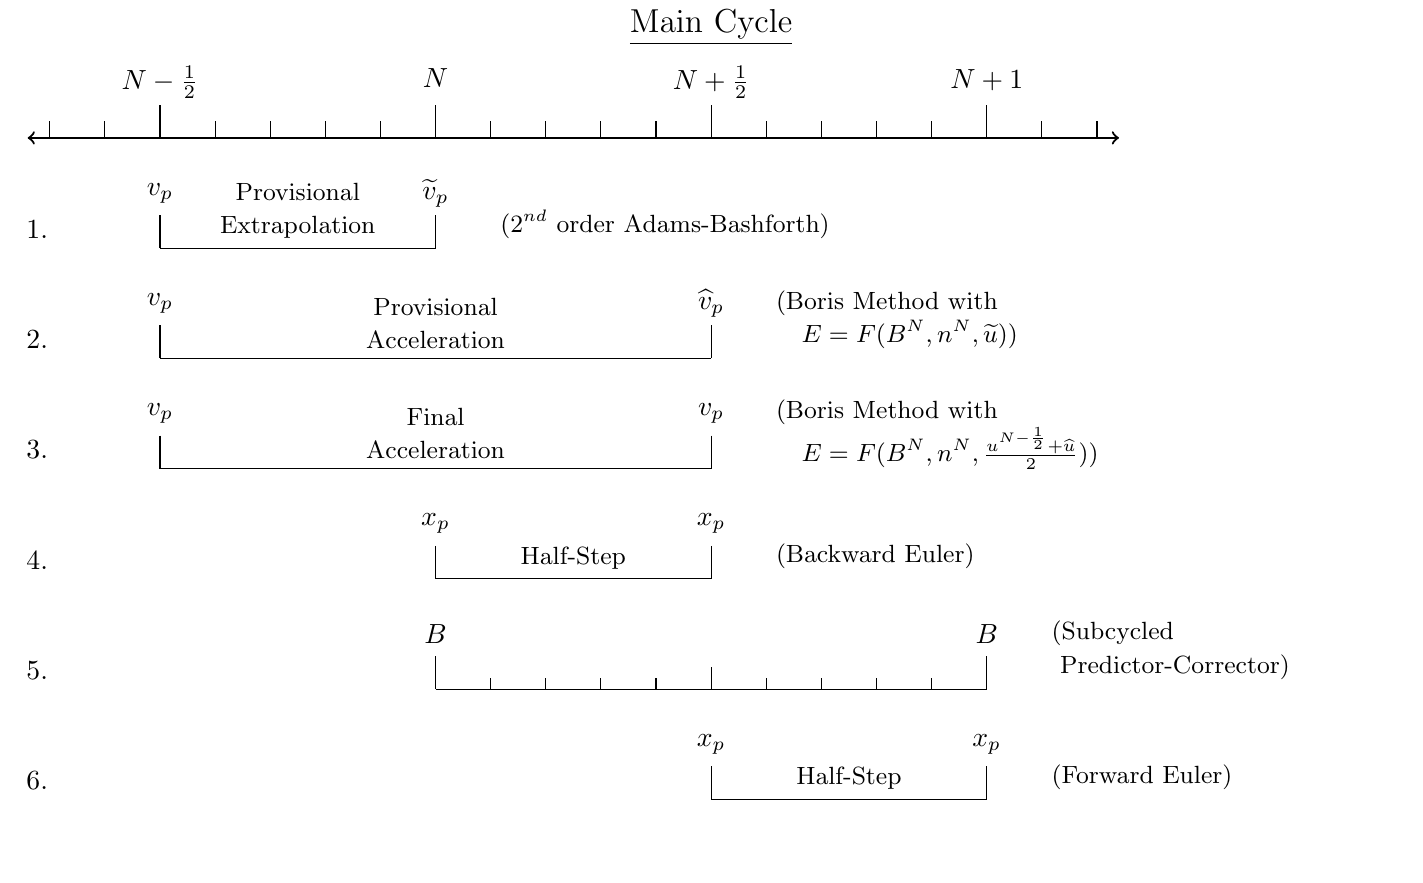
\begin{tikzpicture}[scale=0.7]
%define stuff
\def\left{-7.4}
\def\right{17.4}
\def\gridleft{-7}
\def\gridright{17}
\def\top{10}
\def\bottom{-5}
\def\timeline{8}
%set bounding box
\useasboundingbox (\left,\bottom) rectangle (\right,\top);
%draw background grid (comment when done designing)
%\mygrid[min x=\gridleft, max x=\gridright, min y=\bottom, max y=\top, color=gray]
%Make a title
\node[align=center] (title)
	at (current bounding box.north)
	{\large \underline{Main Cycle}};
%Draw main time axis
\foreach \pos in {-7,-6,...,0,1,2,...,12}
{
	\coordinate (A\pos) at (\pos,\timeline);
	\draw (A\pos) -- ($(A\pos)+(0,0.3)$);
}
\foreach \pos in {-5,0,5,10}
{
	\draw (A\pos) -- ($(A\pos)+(0,0.6)$);
}
\node[label={[yshift=7]$N-\frac12$}] at (A-5) {};
\node[label={[yshift=11]$N$}] at (A0) {};
\node[label={[yshift=7]$N+\frac12$}] at (A5) {};
\node[label={[yshift=10]$N+1$}] at (A10) {};
\draw[<->, thick] (\left,\timeline) -- (12.4,\timeline);
%Step 1
\node (vp1) at (-5,7) {$v_p$};
\draw ($(vp1) - (0,0.4)$) -- ($(vp1) - (0,1)$);
\draw (-5,6) -- node[above, align=center] {\small Provisional\\ \small Extrapolation} (0,6);
\node (vptilde) at (0,7) {$\widetilde{v}_p$};
\draw ($(vptilde) - (0,0.4)$) -- ($(vptilde) - (0,1)$);
\node[above right] (extraplabel) at (1,6) {\small ($2^{nd}$ order Adams-Bashforth)};
%Step 2
\node (vp2) at (-5,5) {$v_p$};
\draw ($(vp2) - (0,0.4)$) -- ($(vp2) - (0,1)$);
\draw (-5,4) -- node [above, align=center] {\small Provisional\\ \small  Acceleration} (5,4);
\node (vphat) at (5,5) {$\widehat{v}_p$};
\draw ($(vphat) - (0,0.4)$) -- ($(vphat) - (0,1)$);
\node[above right, align=left] (pacclabel) at (6,4) {\small (Boris Method with\\ \small  \quad $E = F(B^N, n^N, \widetilde{u})$)};
%Step 3
\node (vp3) at (-5,3) {$v_p$};
\draw ($(vp3) - (0,0.4)$) -- ($(vp3) - (0,1)$);
\draw (-5,2) -- node [above, align=center] {\small Final\\ \small  Acceleration} (5,2);
\node (vpfinal) at (5,3) {$v_p$};
\draw ($(vpfinal) - (0,0.4)$) -- ($(vpfinal) - (0,1)$);
\node[above right, align=left] (facclabel) at (6,1.8) {\small (Boris Method with\\ \small  \quad $E = F(B^N, n^N, \frac{u^{N-\frac12} + \widehat{u}}{2})$)};
%Step 4
\node (xp1) at (0,1) {$x_p$};
\draw ($(xp1) - (0,0.4)$) -- ($(xp1) - (0,1)$);
\draw (0,0) -- node [above, align=center] {\small Half-Step} (5,0);
\node (xpf1) at (5,1) {$x_p$};
\draw ($(xpf1) - (0,0.4)$) -- ($(xpf1) - (0,1)$);
\node[above right, align=left] (xp1label) at (6,0) {\small (Backward Euler)};
%Step 5
\node (B1) at (0,-1) {$B$};
\draw ($(B1) - (0,0.4)$) -- ($(B1) - (0,1)$);
\foreach \pos in {1,2,...,9}
{
	\coordinate (Btick\pos) at (\pos,-2);
	\draw (Btick\pos) -- ($(Btick\pos)+(0,0.2)$);
}
\draw (Btick5) -- ($(Btick5)+(0,0.4)$);
\draw (0,-2) -- (10,-2);
\node (B2) at (10,-1) {$B$};
\draw ($(B2) - (0,0.4)$) -- ($(B2) - (0,1)$);
\node[above right, align=left] (Blabel) at (11,-2) {\small (Subcycled\\ \small ~Predictor-Corrector)};
%Step 6
\node (xp2) at (5,-3) {$x_p$};
\draw ($(xp2) - (0,0.4)$) -- ($(xp2) - (0,1)$);
\draw (5,-4) -- node [above, align=center] {\small Half-Step} (10,-4);
\node (xpf2) at (10,-3) {$x_p$};
\draw ($(xpf2) - (0,0.4)$) -- ($(xpf2) - (0,1)$);
\node[above right, align=left] (xp1label) at (11,-4) {\small (Forward Euler)};

% Draw step numbers
\node[above right] (step1) at (-7.6,6) {1.};
\node[above right] (step1) at (-7.6,4) {2.};
\node[above right] (step1) at (-7.6,2) {3.};
\node[above right] (step1) at (-7.6,0) {4.};
\node[above right] (step1) at (-7.6,-2) {5.};
\node[above right] (step1) at (-7.6,-4) {6.};

\end{tikzpicture}

\vspace{0.5in}

\noindent\begin{tikzpicture}[scale=0.7]
%define stuff
\def\left{-7.4}
\def\right{17.4}
\def\gridleft{-7}
\def\gridright{17}
\def\top{10}
\def\bottom{3}
\def\timeline{8}
%set bounding box
\useasboundingbox (\left,\bottom) rectangle (\right,\top);
%draw background grid (comment when done designing)
%\mygrid[min x=\gridleft, max x=\gridright, min y=\bottom, max y=\top, color=gray]
%Make a title
\node[align=center] (title)
	at (current bounding box.north)
	{\large \underline{Subcycle}};
	
%Draw main time axis
\foreach \pos in {-5,2.5,10}
{
	\coordinate (A\pos) at (\pos,\timeline);
	\draw (A\pos) -- ($(A\pos)+(0,0.6)$);
}
\draw[<->, thick] (\left,\timeline) -- (12.4,\timeline);
\node[above] (m-1) at ($(A-5)+(0,0.6)$) {$N + \frac{m-1}{10}$};
\node[above] (m) at ($(A2.5)+(0,0.6)$) {$N + \frac{m}{10}$};
\node[above] (m+1) at ($(A10)+(0,0.6)$) {$N + \frac{m+1}{10}$};
%Predict
\node (B1) at (-5,7) {$B$};
\draw ($(B1) - (0,0.4)$) -- ($(B1) - (0,1)$);
\draw (-5,6) -- node [above, align=center] {\small Predict} (10,6);
\node (Bbar) at (10,7) {$\bar{B}$};
\draw ($(Bbar) - (0,0.4)$) -- ($(Bbar) - (0,1)$);
\node[above right, align=left] (predictlabel) at (11,6) {\small (Leapfrog with\\ \small \quad $E = F(B^{N+\frac{m}{10}}, n^{N+\frac12}, u^{N+\frac12})$)};
%Correct
\node (B2) at (2,5) {$B$};
\draw ($(B2) - (0,0.4)$) -- ($(B2) - (0,1)$);
\draw (2,4) -- node [above, align=center] {\small Correct} (10,4);
\node (Bf) at (10,5) {$B$};
\draw ($(Bf) - (0,0.4)$) -- ($(Bf) - (0,1)$);
\node[above right, align=left] (predictlabel) at (11,4) {\small (Leapfrog with\\ \small \quad $E = F(\frac{B^{N+\frac{m}{10}} + \bar{B}}{2}, n^{N+\frac12}, u^{N+\frac12})$)};
%Step numbers
\node[above right] (step1) at (-7.6,6) {a.};
\node[above right] (step1) at (-7.6,4) {b.};
\end{tikzpicture}

The set of model equations is solved using a Particle-In-Cell (PIC) method where the ion distribution
functions are approximated by macro-particles and the magnetic field is advanced on a Yee grid with 
Faraday's law. At the start of each iteration of the main loop magnetic field values and ion macroparticle
positions are known at the current time step, while velocities are known at the previous half time step.
The simulation is marched forward in time by the following algorithm.
\begin{enumerate}
\item Extrapolate velocities to the current time step using the second order Adams-Bashforth method.
\item Integrate the extrapolated velocities to compute $E$ and use it to advance particle velocities from time step $N-\frac12$ to $N+\frac12$
\item \begin{enumerate}
	\item Average $v^{N-\frac12}$ and $v^{N+\frac12}$ to get an improved estimate of the velocity at time level $N$
	\item Use the improved velocity to compute an improved electric field
	\item Recompute the particle acceleration using the improved electric field
\end{enumerate}
\item Use $v^{N+\frac12}$ to update particle positions by half a time step, to $N+\frac12$
\item Fix $n$ and $u$ at the half time step so that Faraday's law can be advanced as a Method-of-Lines system of ODE's (See subcycle algorithm for the details of the ODE solver)
\item Use $v^{N+\frac12}$ to update particle positions by another half a time step, to $N+1$
\end{enumerate}

\subsection*{Distribution Function Update}
First, the distribution function is approximated by the sum
\[ f_s(x,v,t) \approx \sum_p N_p S_x(x-x_p(t)) S_v(v-v_p(t)) \]
where each term of the sum represents one macro-particle, a collection of $N_p$ physical particles that
are all near each other in phase space. How near is decided by the so-called shape functions $S_x$ and $S_v$.
the function $S_x$ is chosen to be a zero order b-spline (square cloud) with a width equal to the
grid spacing used for the fields and $S_v$ is chosen to be a delta function.
By requiring that this approximation satisfies the zeroth and first moments of the Vlasov equation
a system of ODEs is derived.
\begin{empheq}[box=\fbox]{align}
\frac{dN_p}{dt} &= 0\\
\frac{dx_p}{dt} &= v_p\\
\frac{dv_p}{dt} &= E + v \times B
\end{empheq}
This system is advanced in time using the Boris method by holding positions at whole time steps and
velocities at half time steps. Sources and sinks can be simulated by adding and removing particles.

\subsection*{Field Update}
The fields are updated using a predictor-corrector method.
Since the timestep is typically most constrained by the magnetic field CFL condition, we
subcycle the field update to get better performance.

The numerical solution is then very similar to standard Particle-In-Cell techniques 
but with a simplified field update and no need to track electron macro-particles.
TODO: Write about the specific field update method


\end{document}
